\appendix

\section{Sensitivity Analysis (H-M4)}

\begin{table}[h]
\centering
\caption{Saturation date error (months) across threshold combinations -- GLUE.}
\begin{tabular}{lccc}
\toprule
$\theta_K$ \textbackslash\ $\theta_r$ & 0.02 & 0.05 & 0.10 \\
\midrule
0.95 & 8 & \textbf{1} & 3 \\
0.99 & 8 & \textbf{3} & 3 \\
1.00 & 20 & 19 & 19 \\
\bottomrule
\end{tabular}
\end{table}

\begin{table}[h]
\centering
\caption{Saturation date error (months) across threshold combinations -- SuperGLUE.}
\begin{tabular}{lccc}
\toprule
$\theta_K$ \textbackslash\ $\theta_r$ & 0.02 & 0.05 & 0.10 \\
\midrule
0.95 & 7 & \textbf{1} & 6 \\
0.99 & 7 & \textbf{5} & 5 \\
1.00 & 10 & 10 & 10 \\
\bottomrule
\end{tabular}
\end{table}

\section{Hyperparameter Configuration}

\begin{verbatim}
# Logistic fitting (H-E1/M2/M3) -- main pipeline
p0 = [0.92, 0.15, 12.0]
bounds_lower = [0.5, 0.01, -24.0]
bounds_upper = [1.05, 3.0, 72.0]
maxfev = 10000
bootstrap_n = 500

# Saturation detection (H-M4)
threshold_k = 0.99
threshold_k_optimal = 0.95
threshold_rate = 0.05
min_monthly_observations = 12

# Boundary condition (H-C1)
bounds_lower_c1 = [0.8, 0.1, 6]
bounds_upper_c1 = [1.0, 2.0, 48]
\end{verbatim}

\section{H-C1 Ablation Results}

\begin{figure}[h]
  \centering
  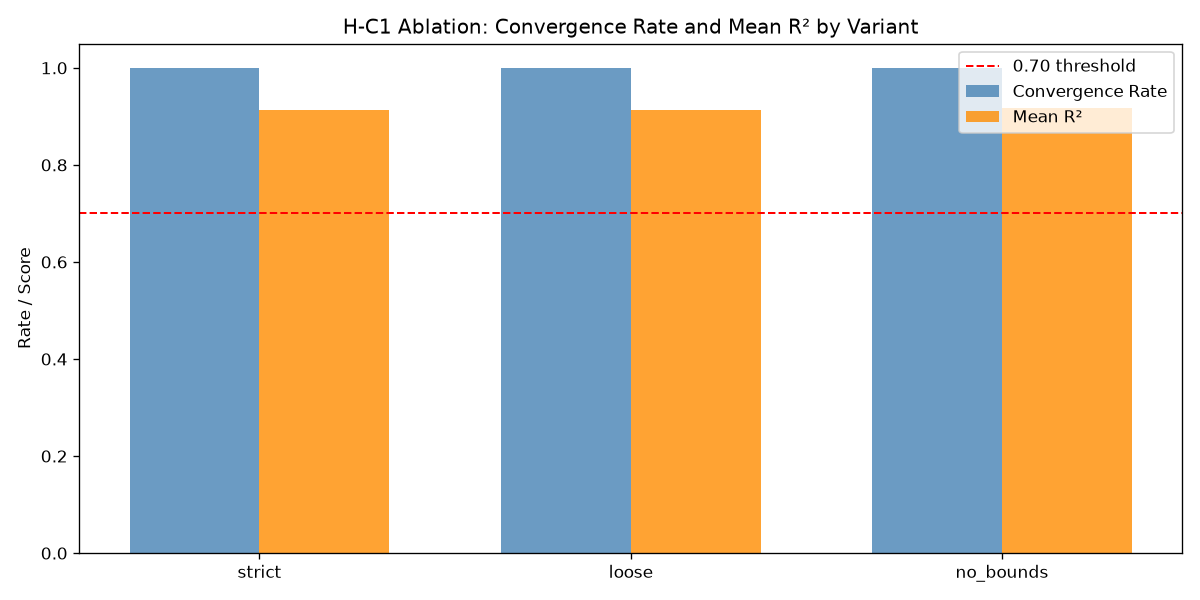
\includegraphics[width=0.48\linewidth]{figures/h-c1_ablation_summary.png}
  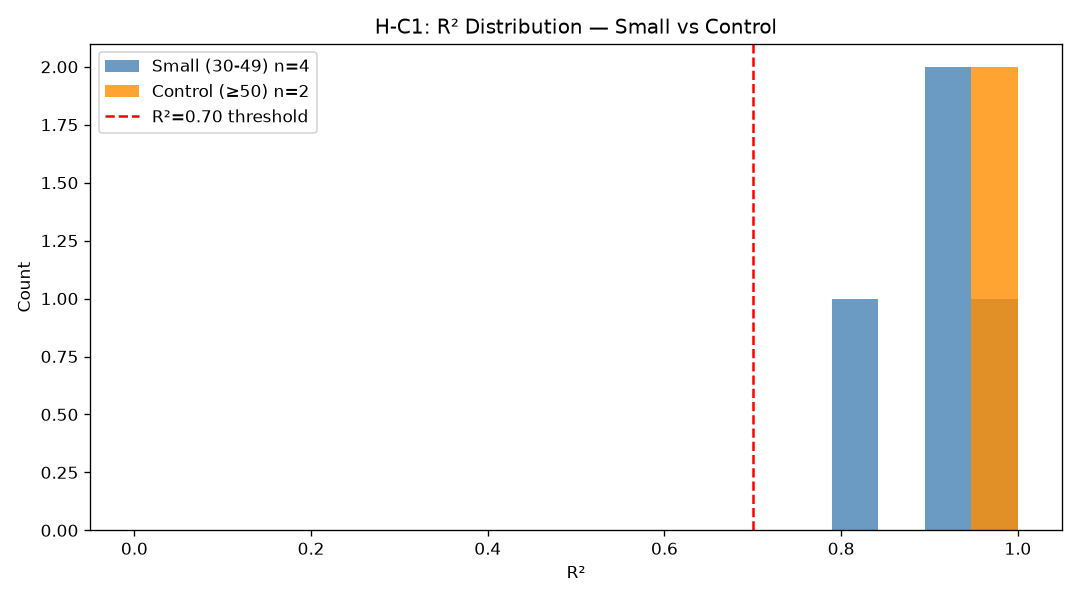
\includegraphics[width=0.48\linewidth]{figures/h-c1_r2_distribution.png}
  \caption{Left: Convergence rate, mean $R^2$, and parameter plausibility across 20 synthetic benchmarks. Right: $R^2$ distribution.}
  \label{fig:ablation_summary}
\end{figure}
